\section{A Distance Sensitive Encoding Protocol}

\subsection{Idea}

In the previous section we discussed various LDP Protocols that function extremely well for numerical values (histogram type), with accuracy that is completely acceptable. However, when the number of users is limited, (eg under 1000), the results of the testings that we carried out are rather alarming, which causes these algorithms to produce inaccurate results. This is mainly due to the fact that the probability of an item to be chosen is independent of the distance between the true and the selected value.


Thus, for the needs of this Thesis, a new L.D.P. protocol was constructed. The idea proposed is to \textbf{have the probability of choosing an element of the domain to depend on the distance from the true value}. This could prove very helpful for histogram values, but does not make any sense for categorical values. From now on, we are going to focus on histogram values.

Based on our idea, the probabilities' distribution, in comparison with the distribution of the D.E. protocol, will look like the one in the following figures.

\begin{figure}[!htb]\centering
    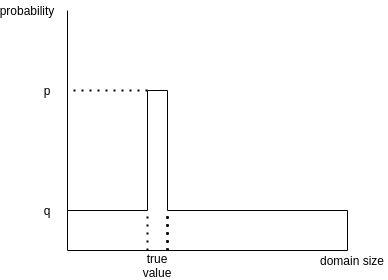
\includegraphics[width=0.5\textwidth]{images/D.E. Idea.png}
    \caption{D.E. protocol's Probabilistic Distribution}
\end{figure}

\begin{figure}[!htb]\centering
    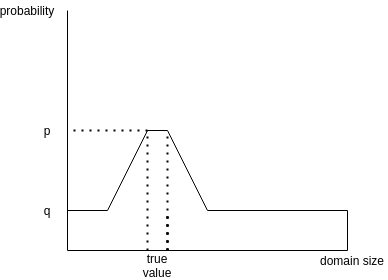
\includegraphics[width=0.5\textwidth]{images/Our Idea.png}
    \caption{Distance Sensitive protocol's Probabilistic Distribution}
\end{figure}


Thus, there is an area around the true value that has high probability to be selected. The width of this area(from now on $\theta$) is defined by the epsilon setting that the user wants to use. The idea for having a specific area and not decreasing our probabilities as low as it goes when we diverge from the true value, is based on our need to be able to serve low epsilon values, as the first would be a big no for when the users wants to use a high privacy setting.

\subsection{Mathematical Background}

In order to achieve our goal, when in the selected area, we must include in the denominator the quantity 
$$
|x - i|
$$
where x is the true value, and the i the false one that we are looking at in order to report it.

When we get out of this area, the denominator will have a constant value, proportional to the boundaries of the selected area. 

\textbf{Example}: Let's suppose that we have a domain size of 100, and our $\theta$ value is 4. All the probabilities outside the area, should be in reverse proportion of $\theta$, thus 4.

Like all probabilistic algorithms though, the sum of the probabilities for all the items in the domain size, must be 1. Thus if we chose the probability to be in the shape of $\frac{a}{|x-i|}$, the partial sum of the series will not give as simple results.

It is known that the series in the form of $a_n = \frac{1}{n}$ does not converge, and its partial sums can only be computed using a complex approximation formula. These characteristics make this type of series very hard to use, and so we have to think of a more handy type.


A type of series that is known to have easy to compute partial sums, are the telescopic series, such as $b_n = \frac{1}{n (n+1)}$. It is known that 
$$
\sum_{n = 1}^{n = k} b_n = 1 - \frac{1}{k + 1}
$$
something that will prove extremely useful moving forward.

So, taking into consideration the quantity $|x - i|$ and the telescopic series $b_n$, we conclude that the probability of each non-true element in our selected area will be of the shape:

\begin{align}
    \mathbf{q = \frac{a}{|x-i|(|x-i| + 1)}}
\end{align}
and outside of that area:

\begin{align}
    \mathbf{s = \frac{a}{\theta \cdot (\theta + 1)}}
\end{align}

The probability $p$ of selecting the true value will have to meet specific criteria that we are going to define later on.

\subsection{Building the Protocol}
Next order of business is to find what the alpha parameter will be, as it is not constant, but obviously it depends on the domain size and the probability $p$. In order to find it, we must keep in mind that all the probabilities of selecting an item from our domain, must add up to $1$.

In order to find out the $\alpha$ value, we must solve the following equation:

\begin{align*}
    p + \sum_{i = x - \theta}^{i = x + \theta} q + \sum_{i = 1}^{i = x - \theta -1} s + \sum_{i = x + \theta + 1}^{i = d} s = 1
\end{align*}

At this point, we must note that $\alpha$ although not a constant, can be held out of the sums, because it is obviously independent from the $i$ variable, that is the variable parsing through the domain in order to retrieve the false elements' probabilities. Thus, we have:

\begin{align*}
        p + \sum_{i = x - \theta}^{i = x + \theta} q + \sum_{i = 1}^{i = x - \theta -1} s + \sum_{i = x + \theta + 1}^{i = d} s = 1 \Longleftrightarrow \\
      \sum_{i = x - \theta}^{i = x + \theta} \frac{a}{|x-i|(|x-i| + 1)} + \sum_{i = 1}^{i = x - \theta -1} \frac{a}{\theta(\theta+1)} + \sum_{i = x + \theta + 1}^{i = d} \frac{a}{\theta(\theta+1)} = 1 - p \Longleftrightarrow \\ \dots \Longleftrightarrow \\ 
    a = \frac{\theta(\theta + 1) (1 - p)}{2\theta^2 - 2\theta + d - 1}
\end{align*}

The proof for the mathematical equations leading to the extraction of the alpha value, can be found in the First Appendix of the Thesis.

\subsection{Epsilon Requirements}

The epsilon value is the most essential in these protocols, as it determines the privacy level that the protocol yields.

Recalling the definition of LDP, we must follow the following rule:

\begin{center}
An algorithm $A$ satisfies \espilon-LDP \textit{iff} for any input $v_1$ and $v_2$, we have
\begin{align*}
    \forall y \in Range(A): \frac{Pr[A(v_1) = y]}{Pr[A(v_2) = y]} \leq e^{\epsilon}
\end{align*}
    
\end{center}

Thus, in order to determine the epsilon value for our algorithm, it must satisfy even the worst case of this equation. The fraction gets bigger, if we put on the biggest probability on the numerator, and the smallest probability of all in the denominator. 

The numerator must have the probability $p$, and the denominator $s$, the probability of all of the elements outside of the $\theta$ area. 

We want for $p$ to be the biggest probability among all, but not extremely high, in order to be able to restrict the growth of epsilon. Hence, we are going to set it as double of the probabilities of its exact neighbours. The 2 neighbours have $|i-x| = 1$, thus $q = \frac{a}{2}$, so we are going to set $\mathbf{p = 2 \cdot \frac{a}{2} = a}$, where $a$ is the quantity defined above, depending on the domain size, and the $\theta$ value.

Now, if we set $p = a$, then the $a$ equation changes, and now our aplha parameter only depends on the domain size and the $\theta$ selected. So, we proceed as following:
\begin{align*}
    a = \frac{\theta(\theta + 1) (1 - p)}{2\theta^2 - 2\theta + d - 1} \Longleftrightarrow{(p = a)}\\
    a = \frac{\theta(\theta + 1) (1 - a)}{2\theta^2 - 2\theta + d - 1} \Longleftrightarrow \\
    a (2\theta^2 - 2\theta + d - 1) = \theta(\theta + 1) - (\theta^2 + \theta)a \Longleftrightarrow\\
    a (3\theta^2 - \theta + d - 1) = \theta(\theta + 1) \Longleftrightarrow \\
    \mathbf{a = \frac{\theta(\theta + 1)}{3\theta^2 - \theta + d - 1}}
\end{align*}

Obviously, we observe the constraint that $\theta > 0$, and this is a special case of our protocol, that can be represented by the direct encoding protocol.

We now have:

\begin{align*}
    \frac{Pr[A(v_1) = y]}{Pr[A(v_2) = y]} = e^{\espilon} \Longleftrightarrow 
    q e^{\epsilon} = p \Longleftrightarrow \\
    \frac{a}{\theta(\theta + 1)} \cdot e^{\epsilon} =  a \Longleftrightarrow \\
    \theta(\theta + 1) = e^{\epsilon} \Longrightarrow \\
    \theta^2 + \theta - e^\epsilon = 0
\end{align*}

If we solve the quadratic equation, and reject its one (illegal) solution, we get that:

\begin{align}
    \theta = \lfloor \frac{\sqrt{4e^{\epsilon} + 1} - 1}{2}\rfloor
\end{align}

So, to conclude, in order for the protocol to function, the user must provide just the epsilon setting, from which the $\theta$ constant is computed, and so the probabilities for each item of the domain to be selected.  


\subsection{Protocol Definition}

We are now ready to define our protocol, by determining the 3 basic operations for an LDP protocol, the \textbf{encoding}, the \textbf{perturbation} and the \textbf{aggregation methods}.


We are going to use the following symbols:
\begin{itemize}
    \item $D$: The protocol's domain. In this set, we have each $i$ for $1 \leq i \leq |D|$ as each item in the domain $D$
    \item $a$: The quantity that we computed in the previous section
    \item $\theta$: The constant used in the previous section, which denotes the area around the true value that the probabilities will be higher than others.
    
\end{itemize}

\textbf{Encoding:} The encoding procedure is trivial. Just like the Wang paper, we are just going to set:
\begin{align*}
    Encode(v) = v
\end{align*}

for each value $v$ of the domain. The values are going to be randomized during the perturbation step.

\textbf{Perturbation:} Given the previous section, the randomization during the perturbation step is define as following:

\begin{equation*}
    Pr[Perturb(x) = i] =
	\begin{cases}
		p = a & \mbox{if } i = x \\
		q = \frac{a}{|c|(|c| + 1)}  &  c = \min{(\theta, |i-x|)}  \mbox{, otherwise}	\end{cases}
\end{equation*}
 
where $i$ is the value selected each time, and $x$ our initial selection. 

\textbf{Aggregation:} The aggregation step was the most tricky during the building of the protocol. A similar approach to the aggregation of pure protocols was chosen, but with a few changes. After several different tries, the optimal aggregation found, was the following: the protocol supports only the reported values corresponding to the true one, thus $Support(v) = v$. However, the $p^*$ quantity is the sum of all the probabilities inside the area: 

\begin{align*}
    p^* = \sum_{x\in (-\theta, \theta)} p(x)
\end{align*}

Finally, the $q*$ quantity is the probability of choosing an element from outside the θ area, thus equal to $s$. Hence, the estimation generated for a value $v$ of the possible answers in the domain is defined as following:

\begin{align*}
    Estimation(v) = \frac{\sum_{j} 1_{support(v^j)}(i) - nq^*}{p^* - q^*}
\end{align*}

\subsection{Extreme Cases}

The downside of a complicated protocol, are of course some extreme cases for the $x, \theta \text{ and } i$ values, all of which we are going to examine in this chapter. The definition of the protocol is going to be altered, and the constraints increased, in order to support those extreme cases.

\textbf{Extreme theta cases:} Of course, we have the constraint that $0 < \theta \leq d$, but what happens when its value is equal to one of the bounds?
\begin{itemize}
    \item When $\theta \leq 0$, our protocol can not function, as this assignment will result in $a = 0$, something that is prohibited, because the probabilities will not sum to 1. In order to ensure that $\theta$ is at least 1, the user must provide at least an $\epsilon = ln(2)$.
    
    \item When $\theta = 1$, we can see that the third case in the perturbation step does not exist, thus we have only the first 2 cases. There, $p = a = \frac{2}{d+1}$, and for every other $i$, $q = \frac{a}{2}$, something that is similar with the Direct Encoding protocol.
    
    \item When $\theta = d$, which realistically can only happen when d is extremely small, then our protocol functions as designed, and has its best behavior. However, if the selection of epsilon results in such big a theta, then the user does not have extreme privacy demands.
\end{itemize}

\textbf{Extreme x values:} Even when the epsilon value and the domain size are normal, in some cases we might face a certain difficulty: if $x - \theta < 0$ or $x + \theta > d$, some of the items in our area are actually outside of our domain boundaries. This results in the sum of the items in the probabilistic distribution to be below 1, something not acceptable. 

In order to fix it, we are going to "transfer" those probabilities inside the boundaries of our domain, while not messing with the highest probability, as this would result in problems with the definition of D.P., an thus the value of theta. 

The idea is to increase the other selections' probabilities by a bit, in order to fill the gap created, while leaving the maximum as initially created. We are going to boost all of the domain's items, by a portion of $\frac{m}{d - 1}$ (as we are altering $d-1$ elements), where $m$ is the sum of the probabilities of the items outside the bounds of our domain. 

However, we are not interested in transferring the whole $Pr[Perturb(x) = i]$, but only its difference from the item with the lowest probability, which is $s =  \frac{a}{\theta(\theta+1)}$. Thus, the $m$ values are defined as following:
\begin{align*}
    m = \sum_{i < 0 \bigcup |i-x|<\theta} Pr[Perturb(x) = i] - \frac{a}{\theta(\theta+1)}
\end{align*}

for the case of $x - \theta < 0$, and as 

\begin{align*}
    m = \sum_{i \geq d \bigcup |i-x|<\theta} Pr[Perturb(x) = i] - \frac{a}{\theta(\theta+1)}
\end{align*}

for the second one.
\\\bigskip
Now, the probabilistic distribution can be altered as following: 


\begin{equation*}
    Pr[Perturb_{DS}(x) = i] =
	\begin{cases}
		p = a & \mbox{if } i = x \\
		q = \frac{a}{|c|(|c| + 1)} + \frac{m}{d - 1}  &  c = \min{(\theta, |i-x|)}  \mbox{, otherwise}	\end{cases}
\end{equation*}
 

The definition of D.P. is not altered, because again in the best case we have a probability of $p = a$, and in the worst case $s = \frac{a}{\theta(\theta+1)}$.

